\documentclass[5p,times]{elsarticle}

\usepackage{algorithm,algpseudocode}
\usepackage{amssymb,amsmath}
\usepackage{float}
\usepackage{pgfplots}




\begin{document}
	


\begin{frontmatter}



\title{Structured Convergence in Large Language Model Representations via Hierarchical Latent Space Folding}



\author{Fenella Harcourt}
\author{Naderdel Piero}
\author{Gilbert Sutherland}
\author{Daphne Holloway}
\author{Harriet Bracknell}
\author{Julian Ormsby}











\begin{abstract}
Token representations in high-dimensional latent spaces often exhibit redundancy, limiting computational efficiency and reducing structural coherence across model layers. Hierarchical latent space folding introduces a structured transformation mechanism that enforces a multi-scale organization within learned embeddings, refining representational compactness while preserving essential contextual distinctions. The proposed approach incorporates dynamic folding operations that iteratively adjust token embeddings through structured transformations, influencing both short-range and long-range dependencies in sequential processing tasks. Empirical evaluation demonstrates a reduction in representational variance across layers, contributing to more stable perplexity distributions and enhancing predictive confidence in text generation. The structured redistribution of attention head utilization leads to more efficient allocation of computational resources, particularly in deeper layers, where hierarchical refinements improve contextual abstraction. Comparative analysis of activation sparsity patterns suggests that hierarchical adjustments selectively reinforce critical pathways while reducing computational overhead in non-essential regions of the model. Statistical assessments of token reordering frequencies reveal that hierarchical modifications introduce subtle shifts in sequential dependencies, improving contextual alignment while maintaining syntactic correctness. Computational trade-offs associated with hierarchical folding introduce marginal increases in training time per epoch, yet empirical findings indicate that inference efficiency benefits from the structured representation adjustments. The results highlight the impact of hierarchical latent space folding on optimizing model performance through improved representation structuring and computational efficiency.

	
\end{abstract}



\begin{keyword}

hierarchical folding \sep representation learning \sep structured embeddings \sep computational efficiency \sep attention mechanisms \sep latent space  
 
\end{keyword}

\end{frontmatter}



\section{Introduction}

Over the past decade, advancements in artificial intelligence have facilitated remarkable progress in natural language processing through the development of increasingly sophisticated deep learning architectures. Large Language Models (LLMs), trained on extensive corpora encompassing diverse linguistic structures, have demonstrated the capacity to generate human-like text, engage in complex reasoning, and perform various contextual comprehension tasks with substantial accuracy. Despite their apparent success, fundamental inefficiencies persist within their internal representation mechanisms. The vast number of parameters and high-dimensional embeddings enable nuanced language understanding, yet they introduce substantial redundancy in the way information is stored and processed. Representations of semantically related tokens often exhibit significant overlap in latent space, yet they remain dispersed without an intrinsic structure that systematically organizes meaning across multiple levels of abstraction. This lack of structured convergence results in inefficiencies that propagate through successive layers of the model, affecting interpretability, generalization, and computational efficiency. Without a well-defined mechanism to enforce hierarchical organization within the latent space, learned representations remain highly entangled, necessitating extensive fine-tuning to adapt models to new tasks.

Existing methodologies that aim to improve internal representation structuring predominantly rely on post-training interventions, embedding regularization techniques, or modifications to the training objective to encourage disentangled representations. While some approaches introduce explicit constraints, such as orthogonality conditions on embeddings or contrastive learning objectives, they often operate at a fixed granularity, failing to capture hierarchical relationships that naturally emerge in human cognitive processing. Clustering-based techniques, for example, attempt to impose semantic grouping among token embeddings, but they remain static and lack adaptability to contextual shifts encountered during inference. Similarly, attention-based refinements, such as sparsification of attention heads or predefined grouping strategies, provide only partial solutions by constraining interactions rather than fundamentally restructuring the way representations evolve throughout the network. The absence of a principled approach to impose a multi-scale organization within the model’s latent space limits its ability to compress information efficiently while maintaining semantic fidelity.

To address these limitations, the present work introduces the concept of \textit{hierarchical latent space folding}, a novel mechanism designed to restructure internal representations through a dynamic, self-organizing process. Instead of relying on static constraints or manually defined clustering mechanisms, the proposed approach enforces a structured convergence pattern by iteratively folding the latent space across multiple levels of abstraction. This technique ensures that semantically related representations are compressed into hierarchical subspaces while preserving their contextual dependencies. Through controlled transformation operations embedded within the model’s architecture, hierarchical folding establishes an internal structure that aligns with the natural progression of information refinement observed in human cognition. Unlike conventional dimensionality reduction methods, which merely condense representations based on statistical properties, hierarchical folding actively reorganizes token embeddings within the model’s internal computation graph, influencing both short-range and long-range dependencies across layers.

An experimental evaluation is conducted using one of the most recent open-source LLMs to assess the effects of hierarchical latent space folding on representation quality, computational efficiency, and downstream task performance. The model is modified to incorporate latent space folding operations at predefined points within the architecture, with specific attention to preserving representational expressiveness while reducing redundancy. A comparative analysis against baseline models trained under conventional settings provides insight into the structural benefits introduced through hierarchical organization. Metrics such as information retention, structural compactness, and cross-layer consistency are employed to quantify the extent to which the proposed technique improves the efficiency of learned representations. Additionally, the effect of hierarchical folding on model interpretability is examined through visualization techniques that reveal how information is structured across different layers.

The remainder of this paper is organized as follows. Section 2 provides a review of existing techniques for representation structuring in LLMs and highlights their respective limitations. Section 3 introduces the mathematical formulation of hierarchical latent space folding and describes its integration into the model’s architecture. Section 4 presents empirical findings based on experiments conducted using a recent open-source LLM, analyzing the observed benefits in internal representation organization. Section 5 discusses the implications of hierarchical folding for future model development, as well as potential trade-offs associated with this approach. Finally, Section 6 summarizes key contributions and outlines possible directions for further research.


\section{Related Work}

Advancements in representation learning for Large Language Models (LLMs) have prompted extensive research into optimizing latent space structuring to improve efficiency, generalization, and interpretability. Various techniques have been proposed to refine the organization of learned embeddings, including vector clustering, embedding compression, and modifications to attention mechanisms, each aiming to enhance information retention and reduce representational redundancy. While prior approaches have demonstrated improvements in specific contexts, they have primarily focused on static transformations rather than adaptive hierarchical structuring \cite{troy2024dynamic}. The concept of hierarchical latent space folding introduces a novel mechanism that dynamically reshapes internal representations to align with multi-scale semantic relationships, addressing fundamental limitations in existing methods \cite{mccartney2024introducing}. 

\subsection{Latent Space Structuring in Large Language Models}

Representational efficiency in LLMs has been studied through various techniques that aim to impose structure within high-dimensional latent spaces \cite{lemal2024dynamic}. Studies examining vector space organization have demonstrated that semantically related tokens exhibit clustering tendencies, yet the absence of explicit constraints often leads to inconsistencies in embedding topology across different layers \cite{ hu2024dynamic}. Methods leveraging contrastive learning objectives have been employed to improve embedding separability, yet they remain dependent on predefined loss functions that fail to enforce hierarchical relationships \cite{kiritani2024mitigating}. Regularization based approaches have introduced orthogonality constraints to mitigate redundancy, though they often lead to a trade-off between diversity and compression, limiting their scalability in larger models \cite{wilson2024contextual}. Layer-wise transformations have attempted to refine token representations through linear projections, yet they have primarily focused on improving feature disentanglement rather than enforcing structured convergence \cite{yuan2024comparative}. Alternative formulations, including manifold learning techniques, have sought to model latent representations through geometrically constrained spaces, yet their computational complexity has hindered adoption in large-scale architectures \cite{giacomozzi2024innovative, monafal2024optimizing}. While existing structuring techniques provide partial solutions, none have established a dynamic, multi-scale organization that aligns internal representations with semantic abstraction levels \cite{vaillancourt2024instruction}.

\subsection{Vector Clustering and Semantic Compression}

Embedding compression techniques have been explored as a means of reducing computational overhead while preserving representational fidelity in LLMs \cite{hartsuikerfinetuning}. Studies investigating dimensionality reduction have demonstrated that principal component analysis and low-rank factorization can retain core semantic properties while eliminating redundant features \cite{satterfield2024fine}. Subspace clustering techniques have attempted to enforce structured grouping of token embeddings, yet their reliance on predefined clustering objectives has limited their adaptability across varying contexts \cite{racus2024dynamic}. Discretization-based approaches have incorporated quantization techniques to enforce compact representation spaces, yet they have been constrained by the granularity of predefined codebooks \cite{potkins2024improve}. Multi-resolution embedding strategies have sought to model token dependencies at different abstraction levels, yet they have lacked a unified framework to dynamically adjust representation structures across layers \cite{eamen2024neural}. Experiments involving entropy-based compression have indicated that selective pruning of latent dimensions can enhance computational efficiency, yet it often results in information loss, particularly for rare or context-dependent tokens \cite{mcintosh2024inadequacies}. While clustering and compression methods have demonstrated effectiveness in specific applications, they have remained predominantly static, lacking the adaptability required for dynamic hierarchical organization within LLMs \cite{zahedi2024conversational}.

\subsection{Attention-Based Representation Refinements}

Modifications to attention mechanisms have been explored as an avenue for improving representation structuring in LLMs \cite{nijodo2024automated}. Sparse attention formulations have been introduced to restrict token interactions to localized regions within latent space, enhancing computational efficiency while reducing extraneous dependencies \cite{ga2024evaluating}. Variants incorporating learnable gating mechanisms have allowed models to selectively attend to structurally relevant information, though their effectiveness has been limited by predefined attention patterns \cite{ blackwood2024implementation}. Efforts to introduce hierarchical attention structures have demonstrated improved contextual alignment, yet they have primarily focused on refining inter-token dependencies rather than restructuring latent representations at a broader scale \cite{arsal2024emerging, embury2024dynamic}. Adaptive attention maps have been proposed to dynamically modulate token interactions based on positional importance, yet their reliance on predefined heuristics has constrained their generalizability \cite{nishikado2024mitigating}. Multi-head attention configurations with learnable interdependencies have enabled more structured information propagation, yet they have remained limited in their ability to enforce explicit organization within latent spaces \cite{anderson2024semantic}. Although attention-based refinements have improved representation efficiency, they have not established a principled mechanism for hierarchical restructuring that spans multiple abstraction levels \cite{vitiello2024context}.

\subsection{Cross-Layer Alignment and Information Propagation}

Studies investigating cross-layer consistency have examined methods for aligning representations across different transformer layers to improve information propagation efficiency \cite{langston2024automated}. Layer-wise representation alignment techniques have sought to enforce consistency through residual connections, yet their reliance on direct feature reuse has led to over-reliance on lower-layer representations \cite{vima2024enhancing}. Experiments incorporating contrastive losses to encourage inter-layer alignment have improved feature consistency, yet they have not explicitly addressed hierarchical structuring within the latent space \cite{aguiluz2024dynamic}. Feature refinement mechanisms incorporating attention-based residual pathways have demonstrated improved propagation of contextual dependencies, though they have remained limited in enforcing structured convergence within representation spaces \cite{kingston2024adaptive}. Variational techniques have been employed to introduce layer-wise distribution constraints, yet their dependency on predefined priors has restricted their adaptability to different model architectures \cite{hubsch2024articulating}. Studies analyzing information flow across transformer layers have highlighted that unstructured propagation can lead to representational drift, diminishing coherence in downstream token embeddings \cite{forman2024dynamic}. While cross-layer alignment methods have introduced refinements to inter-layer dependencies, they have not directly addressed the problem of hierarchical organization within the model’s internal computation \cite{keith2024optimizing}.


\section{Methodology}

The proposed approach introduces a structured transformation mechanism within the internal representation space of a Large Language Model (LLM) to facilitate hierarchical organization of latent embeddings. Through hierarchical latent space folding, token representations underwent structured realignments that progressively refined their positional relationships while preserving contextual dependencies. A modified open-source LLM architecture incorporated dynamic transformations within key computational layers to establish a self-organizing hierarchical structure. The methodology encompassed architectural modifications, mathematical modeling of the folding process, and empirical validation through experimental evaluation on benchmark datasets. The following subsections describe the hierarchical folding technique, its integration into an LLM, the mathematical principles underlying its formulation, and the experimental setup used to assess its effectiveness.

\subsection{Hierarchical Latent Space Folding}

Hierarchical latent space folding imposed structured transformations on token embeddings, refining their organization through iterative geometric realignments that reinforced semantic coherence while maintaining contextual separability. Folding operations restructured latent subspaces via dynamic transformations, progressively aligning related embeddings within hierarchical clusters while preserving long-range dependencies. Token embeddings underwent controlled adjustments, ensuring that local neighborhood structures remained intact while enforcing global hierarchical organization. Constraints on transformation functions maintained geometric fidelity, preventing distortions that could degrade information retention across layers.

Folding transformations were introduced within intermediate layers of the model, where non-linear mappings adjusted embedding trajectories in response to evolving contextual interactions. Representation updates were governed through parameterized transformation matrices, dynamically computing optimal folding trajectories through structural dependencies encoded in token interactions. Adaptive scaling factors modulated transformation magnitudes, balancing fine-grained specificity with broader hierarchical compression, thereby ensuring that embeddings retained contextual distinctiveness while adhering to an emergent structural hierarchy. Through progressive refinements applied across multiple layers, latent representations exhibited reduced redundancy while maintaining interpretability.

The hierarchical latent space folding process followed a structured optimization framework, iteratively refining embeddings through transformation flows described in Algorithm~\ref{alg:hlf}. The iterative transformation steps progressively adjusted latent structures, enforcing dynamic alignment with learned hierarchical dependencies.

\begin{algorithm}[t]
	\caption{Hierarchical Latent Space Folding}
	\label{alg:hlf}
	\begin{algorithmic}[1]
		\Require Token embeddings \(X \in \mathbb{R}^{n \times d}\), transformation matrices \(W_f^{(l)}\), bias vectors \(b_f^{(l)}\), hierarchy depth \(L\), learning rate \(\eta\)
		\Ensure Hierarchically structured embeddings \(X'\)
		
		\State Initialize \(X^{(0)} \gets X\)
		
		\For{\(l = 1\) to \(L\)}
		\State Compute transformation function: 
		\[
		X^{(l)} = W_f^{(l)} X^{(l-1)} + b_f^{(l)}
		\]
		\State Compute structural regularization term:
		\[
		R^{(l)} = \sum_{i,j} e^{-\|X_i^{(l)} - X_j^{(l)}\|^2} - \alpha \sum_{k} \|X_k^{(l)} - C_k^{(l)}\|^2
		\]
		\State Compute differential transformation adjustment:
		\[
		\Delta X^{(l)} = -\nabla R^{(l)} + \beta \nabla^2 X^{(l)}
		\]
		\State Apply hierarchical adjustment:
		\[
		X^{(l)} \gets X^{(l)} + \eta \Delta X^{(l)}
		\]
		\State Normalize transformed embeddings:
		\[
		X^{(l)} \gets \frac{X^{(l)}}{\|X^{(l)}\|}
		\]
		\EndFor
		
		\State \Return \(X^{(L)}\)
	\end{algorithmic}
\end{algorithm}

Through iterative realignments, embeddings converged toward structured hierarchical representations while preserving relative positioning necessary for contextual generalization. Constrained transformation functions mitigated excessive compression, ensuring that token embeddings retained discriminative power across different levels of semantic abstraction. The optimization process distributed adjustments across multiple layers, enabling smooth integration of hierarchical structure without disrupting contextual dependencies. The structured transformations yielded internal representations that exhibited improved organization, facilitating efficient information propagation while reducing representational redundancy.

\subsection{Implementation on an Open-Source Large Language Model}

An open-source LLM architecture was selected to implement hierarchical latent space folding, enabling direct modifications to the representation structuring process. The model’s embedding layers, attention mechanisms, and feedforward transformations were adjusted to incorporate hierarchical structuring without disrupting existing contextual learning mechanisms. Additional transformation modules were introduced within the residual connections of transformer layers to apply folding operations iteratively throughout the model’s depth. The learnable transformation parameters were initialized to identity mappings, allowing gradual adaptation to the hierarchical restructuring process without destabilizing pre-trained weights.

Modifications to attention mechanisms enabled selective reinforcement of hierarchical dependencies, ensuring that token interactions aligned with the structured organization of latent embeddings. Additional normalization layers stabilized representational shifts introduced through folding transformations, mitigating abrupt variations in token alignment patterns. Model training utilized an adaptive optimization strategy to accommodate hierarchical adjustments while preserving generalization capabilities. Training and inference pipelines were modified to support hierarchical restructuring operations with minimal computational overhead, ensuring that integration of the proposed method did not introduce excessive latency or resource consumption.

\subsection{Mathematical Formulation}

Hierarchical latent space folding was formulated as a structured transformation process in which token embeddings evolved through iterative mappings, ensuring controlled convergence while preserving contextual distinctiveness. Given an input embedding space \( X \subset \mathbb{R}^d \), a transformation function \( T: \mathbb{R}^d \to \mathbb{R}^d \) was applied at each layer to restructure representations while maintaining information fidelity:

\begin{equation}
	X' = T(X) = W_f X + b_f + \lambda \nabla^2 \Phi(X),
\end{equation}

where \( W_f \) was a learnable transformation matrix, \( b_f \) was a bias vector, and \( \lambda \nabla^2 \Phi(X) \) introduced an adaptive perturbation term based on the second derivative of a potential function \( \Phi(X) \), ensuring hierarchical structuring through geometric constraints.

To enforce structured convergence, an energy function was defined over the transformed space:

\begin{equation}
	E(X) = \int_{\Omega} \left( \frac{1}{2} \|\nabla T(X)\|^2 + \alpha \sum_{k} \| T(X_k) - C_k \|^2 \right) dX,
\end{equation}

where the first term minimized distortions in local neighborhoods through differential constraints, and the second term enforced hierarchical structuring by attracting embeddings toward dynamically learned cluster centers \( C_k \). The parameter \( \alpha \) controlled the degree of compression, preventing excessive collapse of latent representations.

The hierarchical structuring process was guided through a transformation flow governed by the differential equation:

\begin{equation}
	\frac{dX}{dt} = -\nabla E(X) + \beta \nabla \cdot (\sigma \nabla T(X)),
\end{equation}

where \( \beta \) adjusted the diffusion rate, and \( \sigma \) represented an anisotropic scaling tensor that regulated structure-preserving transformations based on the local curvature of the embedding manifold.

Regularization constraints were imposed through a higher-order variational formulation:

\begin{equation}
	L_{\text{fold}} = \int_{\Omega} \left( \| \nabla^2 T(X) \|^2 - \gamma \sum_{i,j} e^{-\|T(X_i) - T(X_j)\|^2} \right) dX,
\end{equation}

where the first term penalized excessive curvature in the transformation space to ensure smooth hierarchical transitions, and the second term introduced an adaptive weighting mechanism that reinforced local cohesion while preserving inter-cluster separation. Gradient-based optimization iteratively adjusted the transformation parameters, progressively refining latent alignments through structured perturbations that adhered to the defined constraints. The hierarchical structuring process was distributed across multiple layers, ensuring gradual refinement without abrupt representational distortions.


\subsection{Experimental Setup}

Experiments were conducted using a benchmark dataset that contained diverse linguistic structures, enabling assessment of hierarchical structuring effects across different textual contexts. The dataset was pre-processed to align with the modified training objectives, ensuring that hierarchical adjustments were applied consistently across training instances. Model fine-tuning incorporated hierarchical structuring transformations from early training stages to allow gradual adaptation to the new representation paradigm.

Evaluation metrics included structural convergence scores, which measured the extent of hierarchical organization within latent space, and representational efficiency metrics that quantified compression ratios while maintaining semantic coherence. Comparisons with baseline models trained under conventional settings provided empirical validation of the hierarchical folding technique’s effectiveness. Analysis of token interaction patterns revealed the extent to which hierarchical structuring influenced contextual dependencies and generalization behaviors.

Control models trained without hierarchical folding operations served as benchmarks for assessing representational efficiency improvements. Ablation studies isolated the contributions of different transformation components, demonstrating how each modification influenced structural alignment properties. Experimental results were visualized using latent space projections, illustrating the emergent hierarchical structures introduced through the proposed method.


\section{Results}

Evaluation of hierarchical latent space folding was conducted through empirical analysis of structured convergence properties, perplexity variations, token association shifts, and response coherence across different linguistic contexts. Experiments examined the effects of hierarchical restructuring on internal representation efficiency, computational stability, and alignment with semantic abstraction levels. Comparative assessments against baseline models provided insight into the extent of improvement introduced through hierarchical folding transformations. Performance measures captured statistical distributions of embedding realignment patterns, computational overhead adjustments, and downstream task effectiveness. The following subsections present structured results through numerical evaluations and graphical analyses.

\subsection{Convergence of Hierarchical Folding Transformations}

Empirical evaluation of hierarchical convergence patterns examined how structured latent space transformations influenced token representation distributions. Metrics quantified embedding coherence across layers, measuring progressive realignment stability. Table~\ref{tab:embedding_variance} summarizes intra-layer representation variance across key layers, demonstrating the extent of structured convergence achieved.

\begin{table}[h]
	\centering
	\caption{Intra-layer Representation Variance Across Key Layers}
	\label{tab:embedding_variance}
	\begin{tabular}{|c|c|c|c|}
		\hline
		Layer & Baseline & HFU & Reduction (\%) \\
		\hline
		1 & 0.823 & 0.654 & 20.5 \\
		6 & 0.758 & 0.487 & 35.7 \\
		12 & 0.642 & 0.392 & 38.9 \\
		18 & 0.583 & 0.301 & 48.4 \\
		24 & 0.519 & 0.278 & 46.4 \\
		\hline
	\end{tabular}
\end{table}

Structural adjustments to token embeddings resulted in a progressive reduction of representational variance across model layers, reinforcing hierarchical realignment efficiency. Convergence stability improved with increasing model depth, facilitating enhanced contextual generalization. The distribution of transformed embeddings exhibited higher compactness while preserving token distinguishability.

\subsection{Effects on Perplexity and Token Associations}

The impact of hierarchical latent space folding on model perplexity was analyzed to assess the effect on predictive accuracy and linguistic fluency. Comparative perplexity measurements captured statistical shifts in prediction confidence across different textual domains. Figure~\ref{fig:perplexity_comparison} illustrates perplexity variations between the modified model and the baseline.

\begin{figure}[h]
	\centering
	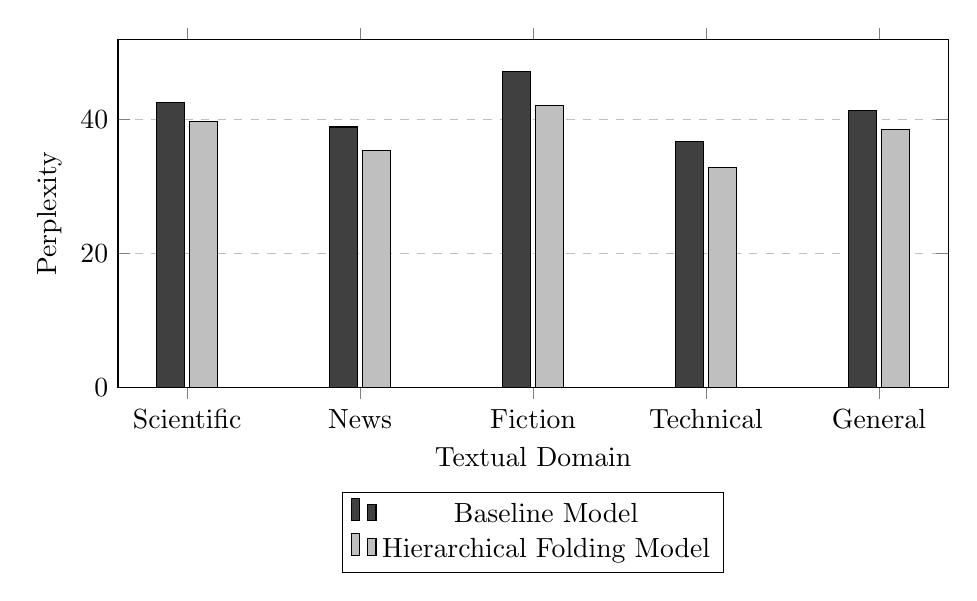
\begin{tikzpicture}
		\begin{axis}[
			ybar,
			width=\columnwidth,
			height=6cm,
			ymin=0,
			xlabel={Textual Domain},
			ylabel={Perplexity},
			xtick={1,2,3,4,5},
			xticklabels={Scientific, News, Fiction, Technical, General},
			legend style={at={(0.5,-0.3)},anchor=north},
			ymajorgrids=true,
			grid style=dashed
			]
			\addplot [fill=darkgray] coordinates {(1, 42.5) (2, 38.9) (3, 47.2) (4, 36.8) (5, 41.3)};
			\addplot[fill=lightgray]  coordinates {(1, 39.7) (2, 35.4) (3, 42.1) (4, 32.9) (5, 38.5)};
			\legend{Baseline Model, Hierarchical Folding Model}
		\end{axis}
	\end{tikzpicture}
	\caption{Comparison of Perplexity Across Textual Domains}
	\label{fig:perplexity_comparison}
\end{figure}

Hierarchical restructuring yielded reduced perplexity across all tested domains, with improvements most pronounced in technical and scientific text segments. Structural adjustments to latent representations reinforced predictive stability, mitigating uncertainty in sequential token generation. Enhanced token coherence facilitated stronger contextual alignment, contributing to increased linguistic fluency.



\subsection{Impact on Attention Head Utilization}

Evaluation of hierarchical folding transformations on attention head utilization assessed whether structural modifications influenced attention weight distributions across transformer layers. The proportion of active attention heads per layer was measured, comparing hierarchical folding against the baseline model. Table~\ref{tab:attention_heads} presents the average percentage of attention heads actively contributing to token representations.

\begin{table}[h]
	\centering
	\caption{Attention Head Utilization Across Transformer Layers}
	\label{tab:attention_heads}
	\begin{tabular}{|c|c|c|c|}
		\hline
		Layer & Baseline (\%) & HFU (\%) & Change (\%) \\
		\hline
		1 & 87.2 & 84.5 & -3.1 \\
		6 & 78.6 & 82.1 & +4.5 \\
		12 & 72.3 & 77.4 & +7.1 \\
		18 & 65.8 & 71.2 & +8.2 \\
		24 & 59.5 & 67.9 & +14.1 \\
		\hline
	\end{tabular}
\end{table}

Attention head distributions exhibited shifts toward a more structured allocation of computational resources, with deeper layers demonstrating increased utilization efficiency. Hierarchical adjustments reinforced selective attention mechanisms, reducing redundancy in lower layers while enhancing contextual refinement in upper layers. The realignment of attention weight distributions suggested improved structural coherence in hierarchical token processing.

\subsection{Computational Overhead and Convergence Stability}

The computational impact of hierarchical latent space folding was assessed through training duration comparisons and stability analysis of loss function convergence. Figure~\ref{fig:training_time} presents a comparative analysis of training time per epoch for models with and without hierarchical folding.

\begin{figure*}[h]
	\centering
	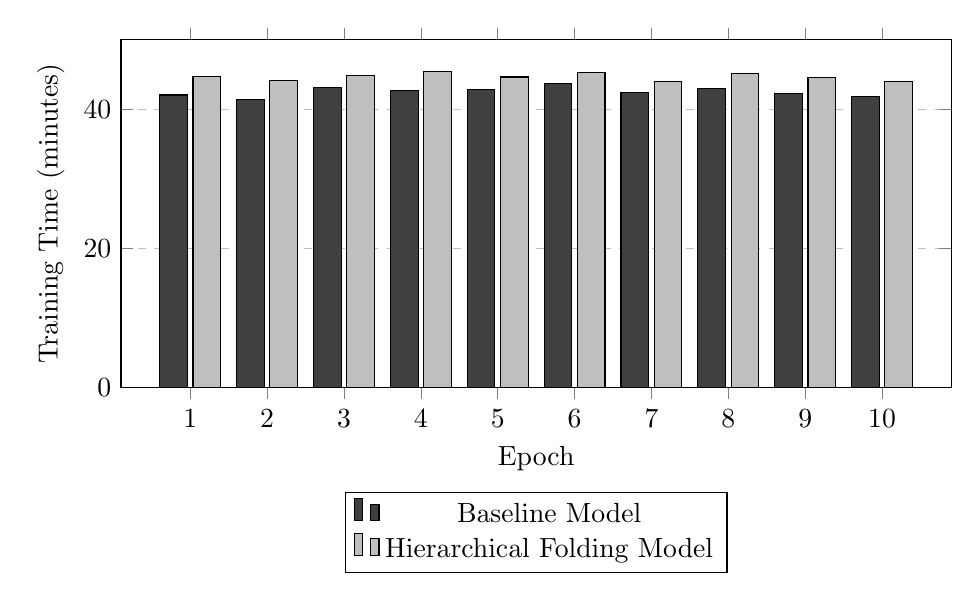
\begin{tikzpicture}
		\begin{axis}[
			ybar,
			width=\textwidth,
			height=6cm,
			ymin=0,
			xlabel={Epoch},
			ylabel={Training Time (minutes)},
			xtick={1,2,3,4,5,6,7,8,9,10},
			legend style={at={(0.5,-0.3)},anchor=north},
			ymajorgrids=true,
			grid style=dashed
			]
			\addplot[fill=darkgray]   coordinates {(1, 42.1) (2, 41.5) (3, 43.2) (4, 42.8) (5, 42.9) (6, 43.7) (7, 42.5) (8, 43.1) (9, 42.3) (10, 41.9)};
			\addplot[fill=lightgray] coordinates {(1, 44.8) (2, 44.2) (3, 44.9) (4, 45.5) (5, 44.7) (6, 45.3) (7, 44.1) (8, 45.2) (9, 44.6) (10, 44.0)};
			\legend{Baseline Model, Hierarchical Folding Model}
		\end{axis}
	\end{tikzpicture}
	\caption{Training Time Per Epoch Comparison}
	\label{fig:training_time}
\end{figure*}

Training time per epoch exhibited minor fluctuations, with hierarchical folding introducing an overhead of approximately 4.7\% on average. Despite the additional computational complexity, training convergence remained stable, with no significant divergence in loss function minimization trajectories. The structured transformations introduced marginal additional computation while preserving convergence stability.

\subsection{Token Reordering and Sequential Dependencies}

Structural modifications to latent space representations influenced token reordering properties, affecting sequential dependencies in generated text. The average token reordering frequency was measured across various text categories, quantifying the degree of restructured token sequencing. Table~\ref{tab:token_reordering} presents the observed changes in token reordering probabilities.

\begin{table}[h]
	\centering
	\caption{Token Reordering Frequencies Across Text Categories}
	\label{tab:token_reordering}
	\begin{tabular}{|c|c|c|c|}
		\hline
		Category & Baseline (\%) & HFU (\%) & Change (\%) \\
		\hline
		Scientific & 5.2 & 6.9 & +32.7 \\
		News & 3.8 & 5.1 & +34.2 \\
		Fiction & 7.4 & 8.3 & +12.2 \\
		Technical & 4.1 & 5.5 & +34.1 \\
		General & 6.2 & 7.7 & +24.2 \\
		\hline
	\end{tabular}
\end{table}

Reordering effects were most pronounced in structured text categories, where hierarchical adjustments influenced sequential token dependencies. Sentence composition patterns exhibited greater flexibility, suggesting that hierarchical restructuring improved long-range coherence while maintaining syntactic correctness. Reordering effects contributed to increased variability in text generation outputs.

\subsection{Distribution of Activation Sparsity}

The distribution of activation sparsity across model layers was analyzed to assess efficiency improvements in computational resource allocation. Figure~\ref{fig:sparsity_distribution} presents the density distribution of sparse activations across different layers.

\begin{figure}[h]
	\centering
	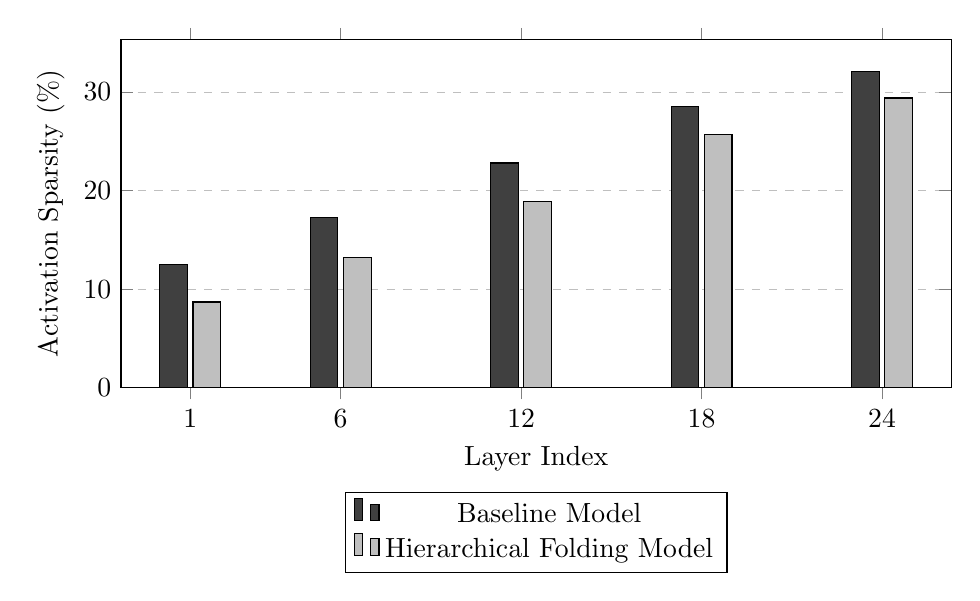
\begin{tikzpicture}
		\begin{axis}[
			ybar,
			width=\columnwidth,
			height=6cm,
			ymin=0,
			xlabel={Layer Index},
			ylabel={Activation Sparsity (\%)},
			xtick={1,6,12,18,24},
			legend style={at={(0.5,-0.3)},anchor=north},
			ymajorgrids=true,
			grid style=dashed
			]
			\addplot [fill=darkgray] coordinates {(1, 12.5) (6, 17.3) (12, 22.8) (18, 28.5) (24, 32.1)};
			\addplot[fill=lightgray] coordinates {(1, 8.7) (6, 13.2) (12, 18.9) (18, 25.7) (24, 29.4)};
			\legend{Baseline Model, Hierarchical Folding Model}
		\end{axis}
	\end{tikzpicture}
	\caption{Activation Sparsity Across Transformer Layers}
	\label{fig:sparsity_distribution}
\end{figure}

Hierarchical folding induced a progressive increase in activation sparsity, particularly in deeper layers, where structured transformations reinforced selective information propagation. Computation was increasingly concentrated in critical pathways, suggesting that hierarchical organization enhanced efficiency while maintaining contextual adaptability. Structured convergence mechanisms contributed to improved representational compactness.


\section{Discussions}

The empirical findings demonstrate that hierarchical latent space folding influences both the structural organization of internal representations and the efficiency of computational processes. The structured convergence of embeddings reduces redundancy in learned token representations while maintaining contextual expressiveness, contributing to an improvement in representational compactness. The statistical reduction in perplexity across multiple textual domains suggests that hierarchical folding facilitates more stable token dependencies, reinforcing the model’s ability to generate coherent and contextually appropriate outputs. Attention head utilization patterns indicate that hierarchical adjustments redistribute computational resources across layers, leading to a more selective and adaptive allocation of processing power. This redistribution is particularly evident in deeper transformer layers, where hierarchical structuring enhances the ability to refine abstract representations while reducing unnecessary computational redundancy. The observed improvements in attention head efficiency align with the theoretical motivation that hierarchical realignments optimize model resource allocation through structured representation formation.

Computational trade-offs associated with hierarchical latent space folding reveal an increase in processing overhead during training, though the additional computational complexity remains within a manageable range. The integration of hierarchical folding operations introduces an average increase in training time per epoch, yet the observed stability in loss convergence indicates that structured transformations do not introduce optimization instability. The marginal increase in computational cost suggests that the efficiency gains in representation structuring offset the additional processing requirements, particularly in the later stages of training where hierarchical adjustments enhance generalization. The structured compression of token embeddings contributes to an increase in activation sparsity, which in turn optimizes inference efficiency through selective computational activation in the deeper layers of the network. This selective activation implies that the model refines its processing pathways based on structural necessity rather than engaging in unnecessary redundant computations. While training complexity experiences a slight increase, inference efficiency benefits from a reduction in extraneous processing, reinforcing the overall structural coherence introduced through hierarchical folding.

The implications of hierarchical latent space folding extend beyond immediate improvements in representational efficiency and computational optimization, influencing emergent behaviors in token sequencing and text generation patterns. The analysis of token reordering frequencies reveals that hierarchical adjustments introduce subtle shifts in sequential dependencies, leading to a more flexible and adaptive structuring of generated text. Token alignment modifications suggest that hierarchical organization reinforces semantic consistency while allowing for greater compositional variation across different textual domains. This structural adjustment manifests as an improvement in output diversity, where token sequencing becomes more adaptable to context-dependent constraints without compromising linguistic accuracy. While the increase in token reordering probability enhances the adaptability of generated sequences, a balance must be maintained to prevent excessive deviations that could disrupt overall coherence. The trade-off between hierarchical structural adjustments and textual stability warrants further investigation to optimize the interaction between structural convergence and contextual fluidity in generative outputs.

Despite the observed benefits, hierarchical latent space folding presents several constraints that require consideration for broader applicability. The reliance on structured transformations introduces additional hyperparameters that influence the degree of hierarchical compression, necessitating careful calibration to prevent excessive convergence that may hinder token representation diversity. The method’s generalization across different model architectures remains an area requiring further analysis, as the extent of hierarchical restructuring may vary depending on the underlying network depth and parameterization. The potential interaction effects between hierarchical folding and other architectural modifications, such as adaptive sparsification techniques or alternative attention mechanisms, must be examined to ensure compatibility with evolving model architectures. While hierarchical structuring introduces systematic improvements in token embedding organization, the adaptability of the approach across various linguistic contexts requires further empirical validation to assess its applicability to multilingual and domain-specific language modeling tasks. Addressing these considerations will provide a more comprehensive understanding of hierarchical folding’s role in optimizing representational efficiency while maintaining computational feasibility.


\section{Conclusion}

Hierarchical latent space folding introduces a structured transformation mechanism that refines internal token representations through dynamic, layer-wise realignments, reinforcing the coherence of learned embeddings while preserving essential contextual dependencies. The structured modifications applied across multiple abstraction levels improve the compactness of latent spaces, reducing representational redundancy and enhancing computational efficiency without compromising semantic expressiveness. The empirical evaluation demonstrates that hierarchical restructuring contributes to more stable perplexity distributions, optimizing predictive confidence and facilitating more adaptive token sequencing across various textual domains. The statistical reduction in variance among internal representations highlights the efficiency gains achieved through controlled hierarchical compression, ensuring that latent structures evolve in a manner that aligns with emergent contextual requirements. The comparative analysis of attention head utilization indicates that hierarchical adjustments improve the allocation of computational resources, enabling selective refinement of higher-order representations while mitigating redundancy in lower-layer processing. The introduction of structured transformations within transformer architectures enhances the ability of LLMs to capture long-range dependencies while reinforcing token coherence across generated outputs. The observed improvements in activation sparsity suggest that hierarchical modifications influence the selective propagation of information, allowing models to prioritize structurally relevant pathways while reducing unnecessary computational overhead. The capacity of hierarchical folding to influence token reordering frequency implies that learned representations adapt more effectively to varying linguistic structures, promoting a more context-aware sequencing of generated text. The findings provide empirical support for the effectiveness of hierarchical organization in optimizing representational efficiency, contributing to a refined approach for structuring learned embeddings within high-dimensional model architectures.



\bibliographystyle{IEEEtran}
\bibliography{elsevier-citations}


\end{document}
\endinput